\documentclass[crop,tikz]{standalone}
\usepackage[utf8]{inputenc}
\usepackage{tikz}
\usepackage{pgfplots}
\usepackage{bm}
\pgfplotsset{compat=newest}
\usepgfplotslibrary{groupplots}
\begin{document}
% This file was created by tikzplotlib v0.8.2.
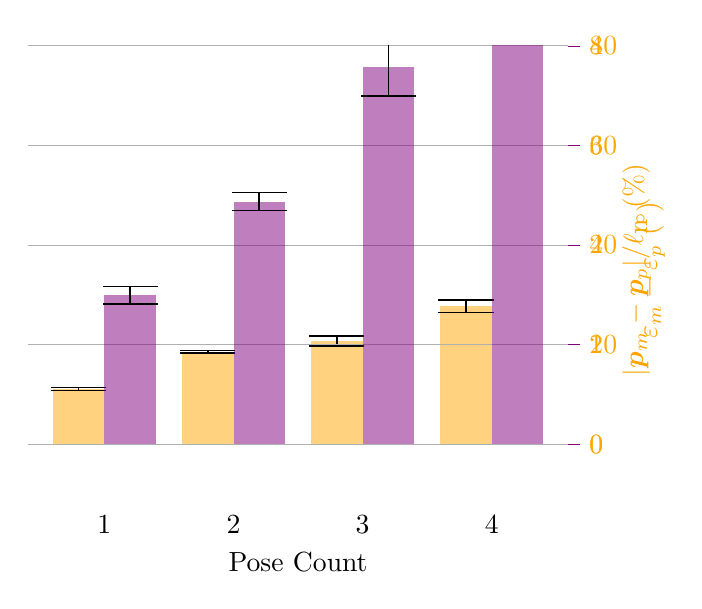
\begin{tikzpicture}
\definecolor{color0}{rgb}{1,0.647058823529412,0}
\definecolor{color1}{rgb}{0.501960784313725,0,0.501960784313725}
\begin{axis}[
anchor=origin,
axis line style={draw=none},
tick align=outside,
tick pos=both,
x grid style={white!69.01960784313725!black},
xmin=-0.59, xmax=3.59,
xtick style={color=black},
xtick style={draw=none},
xtick={0,1,2,3},
xticklabels={ , , , },
y grid style={white!69.01960784313725!black},
ylabel style={color=color0},
ylabel={\(\displaystyle |\bm{p}_m - \bm{p}_p|/\ell_{\textnormal{n}}\) (\%)},
ymin=-0.5, ymax=4,
ytick pos=left,
ytick pos=right,
ytick style={color=color0},
ytick style={color=color0},
yticklabel style={color=color0}
]
\draw[fill=color0,draw opacity=0,fill opacity=0.5] (axis cs:0,0) rectangle (axis cs:-0.4,0.555889632054699);
\draw[fill=color0,draw opacity=0,fill opacity=0.5] (axis cs:1,0) rectangle (axis cs:0.6,0.927791988358189);
\draw[fill=color0,draw opacity=0,fill opacity=0.5] (axis cs:2,0) rectangle (axis cs:1.6,1.03559789298607);
\draw[fill=color0,draw opacity=0,fill opacity=0.5] (axis cs:3,0) rectangle (axis cs:2.6,1.38505318028033);
\path [draw=black, semithick]
(axis cs:-0.2,0.53992191652048)
--(axis cs:-0.2,0.571857347588918);
\path [draw=black, semithick]
(axis cs:0.8,0.914399151558422)
--(axis cs:0.8,0.941184825157956);
\path [draw=black, semithick]
(axis cs:1.8,0.985865111435385)
--(axis cs:1.8,1.08533067453676);
\path [draw=black, semithick]
(axis cs:2.8,1.32442592991916)
--(axis cs:2.8,1.44568043064149);
\addplot [semithick, black, mark=-, mark size=10, mark options={solid}, only marks]
table {%
-0.2 0.53992191652048
0.8 0.914399151558422
1.8 0.985865111435385
2.8 1.32442592991916
};
\addplot [semithick, black, mark=-, mark size=10, mark options={solid}, only marks]
table {%
-0.2 0.571857347588918
0.8 0.941184825157956
1.8 1.08533067453676
2.8 1.44568043064149
};
\end{axis}
\begin{axis}[
anchor=origin,
axis line style={draw=none},
axis y line=right,
tick align=outside,
tick pos=both,
x grid style={white!69.01960784313725!black},
xlabel={Pose Count},
xmin=-0.59, xmax=3.59,
xtick style={color=black},
xtick style={draw=none},
xtick={0,1,2,3},
xticklabels={1,2,3,4},
y grid style={white!69.01960784313725!black},
ylabel style={color=color0},
ylabel={\(\displaystyle \varepsilon_m - \varepsilon_p\) (\(\displaystyle ^\circ\))},
ymajorgrids,
ymin=-10, ymax=80,
ytick pos=left,
ytick pos=right,
ytick style={color=color0},
ytick style={color=color1},
yticklabel style={color=color0}
]
\draw[fill=color1,draw opacity=0,fill opacity=0.5] (axis cs:0,0) rectangle (axis cs:0.4,29.8975713676033);
\draw[fill=color1,draw opacity=0,fill opacity=0.5] (axis cs:1,0) rectangle (axis cs:1.4,48.7427976986753);
\draw[fill=color1,draw opacity=0,fill opacity=0.5] (axis cs:2,0) rectangle (axis cs:2.4,75.7971209195689);
\draw[fill=color1,draw opacity=0,fill opacity=0.5] (axis cs:3,0) rectangle (axis cs:3.4,90.2288515117855);
\path [draw=black, semithick]
(axis cs:0.2,31.6872198758794)
--(axis cs:0.2,28.1079228593273);
\path [draw=black, semithick]
(axis cs:1.2,50.5198763748186)
--(axis cs:1.2,46.965719022532);
\path [draw=black, semithick]
(axis cs:2.2,81.6520989518829)
--(axis cs:2.2,69.9421428872549);
\path [draw=black, semithick]
(axis cs:3.2,94.3593978777457)
--(axis cs:3.2,86.0983051458253);
\addplot [semithick, black, mark=-, mark size=10, mark options={solid}, only marks]
table {%
0.2 31.6872198758794
1.2 50.5198763748186
2.2 81.6520989518829
3.2 94.3593978777457
};
\addplot [semithick, black, mark=-, mark size=10, mark options={solid}, only marks]
table {%
0.2 28.1079228593273
1.2 46.965719022532
2.2 69.9421428872549
3.2 86.0983051458253
};
\end{axis}
\end{tikzpicture}
%% End matplotlib2tikz content %% 
\end{document}